%%%%%%%%%%%%%%%%%%%%%%%%%%%%%%%%%%%%%%%%%%%%%%%%%%%%%%%%%%%%%%%%%%% 
%                                                                 %
%                            CHAPTER                              %
%                                                                 %
%%%%%%%%%%%%%%%%%%%%%%%%%%%%%%%%%%%%%%%%%%%%%%%%%%%%%%%%%%%%%%%%%%% 

%\chapter{Vormelijke richtlijnen van de scriptie}
\chapter{Situering en doelstelling}

\section{Situering}
Tegenwoordig wordt deep learning steeds meer en meer gebruikt om beeldverwerkingsproblemen op te lossen. 
Via neurale netwerken kunnen we met meer en betere features werken om de afbeeldingen te analyseren. 
Veel van deze modellen hebben echter behoorlijk wat rekenkracht en geheugen nodig om te werken.
Bovendien is er steeds meer interesse naar real-time toepassingen waarvan het resultaat zo snel mogelijk beschikbaar moet zijn.
Een voorbeeld hiervan zijn zelfrijdende auto's.
Een zelfrijdende auto moet kunnen stoppen voor een persoon die de weg oversteekt.
Hierbij moet zo snel en accuraat mogelijk een persoon herkend worden zodat de auto op tijd kan stoppen.
Dit wordt moeilijk bij toepassingen waarbij de foto eerst genomen moet worden en vervolgens door een computer geanalyseerd moet worden.
Dit probleem zou nog groter worden wanneer de computer zich op een andere locatie bevindt.
Waardoor we de afbeelding over een internet connectie moeten communiceren.
Dit is omdat huidige herkenningsystemen en detectiesystemen veel rekenwerk en geheugen vragen, het volgende voorbeeld is een mogelijke use-case (figuur :\ref{fig:use_case}). 

\begin{figure}[!ht]
	\centering
	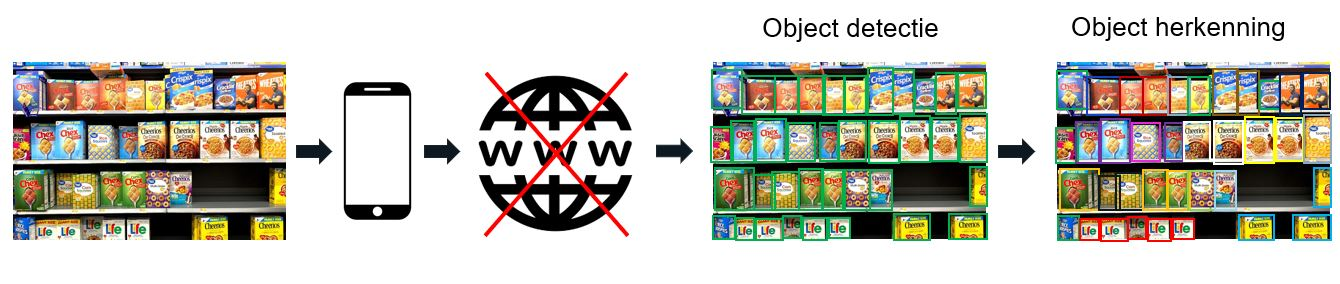
\includegraphics[width=1.0\linewidth]{fig/situering.jpg}
	\caption{Use-case om verschillende producten in winkelrekken te herkennen.}
	\label{fig:use_case}
\end{figure}

Het automatisch detecteren en herkennen van producten in de rekken van een supermarkt heeft veel interessante real-time toepassingen.
Het kan slechtzienden helpen om snel de producten te vinden die ze nodig hebben. 
Het winkelmanagement kan zo een real-time status krijgen van de inventaris op de winkelrekken.
Er kan ook nagekeken worden of de producten staan waar ze horen te staan in de rekken.
Eerdere studies hebben reeds het potentieel van diep neurale netwerken laten zien voor deze taken.
Achter het neuraal netwerk van deze toepassing zit echter veel complex rekenwerk en vereisten voor het geheugen.
Deze beperkingen zorgen voor een groot struikelblok voor real-life toepassingen.
Het zou namelijk handig zijn dat het neuraal netwerk kan worden uitgevoerd op een smartphone.
De voornaamste manier om zware neurale netwerken uit te voeren op een smartphone is door het neuraal netwerk uit te voeren op een server zoals de cloud.
Een internet connectie is nodig om data naar de cloud te sturen en van de cloud te ontvangen.
Door het neuraal netwerk op een smartphone uit te voeren is er geen nood meer aan een internet connectie.
Dit zorgt ook voor een lagere respons tijd omdat de applicatie niet meer moet wachten op het antwoord van het neuraal netwerk dat in de cloud wordt uitgevoerd.
De data blijft zo op de smartphone en wordt niet over het internet gecommuniceerd wat zorgt voor een betere privacy en veiligheid. 
In deze masterproef onderzoeken we hoe een bestaand neuraal netwerk kan worden aangepast, zodat dit bruikbaar is voor een mobiele implementatie.

\section{Probleemstelling}
Mobiele apparaten zijn kleine toestellen met een beperkt geheugen en een beperkte rekenkracht. 
In deze masterproef wordt er onderzocht we het rekenwerk kunnen beperken zodat het resultaat real-time geleverd kan worden. 
We gaan ook onderzoeken hoe alle data effici\"ent kan worden opgeslagen op het toestel. 
Ook zijn niet alle operaties van het neuraal netwerk compatibel met de hardware en software van het mobiele toestel en de applicatie. 

Bij deze masterproef willen we van een neuraal netwerk dat in een bepaald framework gemodelleerd en getraind is gaan naar een mobiele implementatie.
Zo wordt er voor een aantal verschillende frameworks onderzocht op welke manieren deze naar een mobiele implementatie kunnen gaan.
Bovendien zullen we per framework de omzetting naar mobiele implementatie voor verschillende CNN-architecturen onderzoeken. 
Vervolgens zal er ook gekeken worden naar verdere optimalisaties voor herkenningssystemen en detectiesystemen. 
Het uiteindelijke doel is een prototype ontwikkelen dat een bestaand herkenningsnetwerk en detectienetwerk implementeert op een mobiel apparaat. 
Bij dit prototype is dan het rekenwerk en de geheugen vereisten geminimaliseerd zonder een groot effect te hebben op de accuraatheid van het model.

In deze masterproef zal het vooral gaan over het vervangen van operaties in het neuraal netwerk die compatibel zijn met de omgeving waar de mobiele applicatie wordt uitgevoerd.
We gaan ervan uit dat in deze masterproef het model van het neuraal netwerk reeds gemodelleerd en getraind is.


\section{Doelstellingen}
Het doel van deze masterproef is het onderzoeken van de compatibiliteit tussen de operaties van een bestaand neuraal netwerk in zijn originele omgeving en een mobiele omgeving.
Zodat een bestaand en complex deep learning model ge\"implementeert kan worden op een mobiel apparaat met zo min mogelijk effect op de accuraatheid. 
Dit gebeurt aan de hand van de volgende stappen:
\begin{itemize}
    \item Het bespreken van een deep learning herkenningssysteem en detectiesysteem.
    \item Bespreken van frameworks/bibliotheken waarin het basismodel ontwikkeld kan worden.
    \item Bespreken van frameworks, compatibiliteit tussen frameworks en optimalisatietechnieken die ervoor kunnen zorgen dat bestaande modellen mogelijk kunnen uitgevoerd worden op een mobiel apparaat.
    \item De gevonden technieken testen en analyseren voor verschillende frameworks en neurale netwerken met als doel een werkend prototype te ontwikkelen.
\end{itemize}